\section{Building a Roller Coaster}
\label{sec:building_a_roller_coaster}

\subsection*{Recommended Tutorials:}
\begin{itemize}[noitemsep]
	\item \nameref{chp:assignment_operator}, pg. \pageref{chp:assignment_operator}
	\item \nameref{chp:equation_solvers}, pg. \pageref{chp:equation_solvers}
	\item \nameref{chp:derivative}, pg. \pageref{chp:derivative}
\end{itemize}

\subsection*{Introduction:}
You are in charge of designing the first hill of a new roller coaster. For an initial design, you connect a straight stretch of track for the lift hill followed by two parabolas, as shown in Figure \ref{fig:rollercoaster}.

\begin{figure*}[h]
\label{fig:rollercoaster}
\hspace{-3cm}
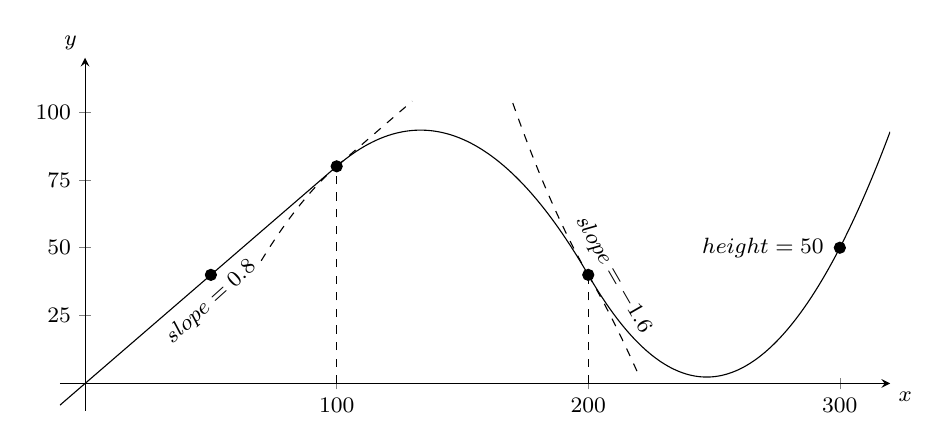
\begin{tikzpicture}
\footnotesize
\begin{axis}[
	width=\textwidth,
	height=0.5\textwidth,
	axis lines=middle,
	xlabel={$x$},
	ylabel={$y$},
	xlabel style={below right},
	ylabel style={above left},
	xmin=-10, xmax=320, xtick={0,100,200,300},
	ymin=-10, ymax=120, ytick={0,25,50,75,100}
]
	\addplot [domain=-10:100, samples=100] {0.8*x};
	\addplot [domain=100:130, samples=100, dashed] {0.8*x};
	\addplot [domain= 70:100, samples=100, dashed] {(-0.012)*x^2+3.2*x-120};
	\addplot [domain=100:200, samples=100] {(-0.012)*x^2+3.2*x-120};
	\addplot [domain=200:220, samples=100, dashed] {(-0.012)*x^2+3.2*x-120};
	\addplot [domain=170:200, samples=100, dashed] {0.017*x^2+((-1)*8.4)*x+1040};
	\addplot [domain=200:320, samples=100] {0.017*x^2+((-1)*8.4)*x+1040};
	\addplot[mark=*] coordinates {(50,40)};
	\draw [dashed] (axis cs:100,0) -- (axis cs:100,80);
	\addplot[mark=*] coordinates {(100,80)};
	\draw(axis cs:50,30) node [rotate=42] {$slope = 0.8$};
	\addplot[mark=*] coordinates {(200,40)};
	\draw [dashed] (axis cs:200,0) -- (axis cs:200,40);
	\draw(axis cs:210,40) node [rotate=-60] {$slope = -1.6$};
	\addplot[mark=*] coordinates {(300,50)} node [left] {$height=50~$};
\end{axis}
\end{tikzpicture}
\caption{A simple design for the initial hill of a roller coaster.}
\end{figure*}
% OLD PSTRICKS CODE
%	\psset{xunit=1.2pt,yunit=1.2pt}
%	\begin{pspicture}(-10,120)(320,-10)
%	\psaxes[ticksize=-2pt 2pt,Dx=50,Dy=20]{->}(0,0)(-10,-10)(320,120)
%	\psplot[algebraic=true,VarStep=true,showpoints=false,plotpoints=100,linewidth=1.0pt]{-10}{100}{0.8*x}
%	\psplot[algebraic=true,VarStep=true,showpoints=false,plotpoints=100,linewidth=1.0pt,linestyle=dashed]{100}{130}{0.8*x}
%	\psplot[algebraic=true,VarStep=true,showpoints=false,plotpoints=100,linewidth=1.0pt,linestyle=dashed]{70}{100}{(-0.012)*x^2+3.2*x-120}
%	\psplot[algebraic=true,VarStep=true,showpoints=false,plotpoints=100,linewidth=1.0pt]{100}{200}{(-0.012)*x^2+3.2*x-120}
%	\psplot[algebraic=true,VarStep=true,showpoints=false,plotpoints=100,linewidth=1.0pt,linestyle=dashed]{200}{220}{(-0.012)*x^2+3.2*x-120}
%	\psplot[algebraic=true,VarStep=true,showpoints=false,plotpoints=100,linewidth=1.0pt,linestyle=dashed]{170}{200}{0.017*x^2+((-1)*8.4)*x+1040}
%	\psplot[algebraic=true,VarStep=true,showpoints=false,plotpoints=100,linewidth=1.0pt]{200}{320}{0.017*x^2+((-1)*8.4)*x+1040}
%	\psline(100,0)(100,80)
%	\psline(200,0)(200,40)
%	\psline(300,0)(300,50)
%	\end{pspicture}
\noindent
The following criteria must be met to build the roller coaster:
\begin{itemize}
	\item The lift hill will have a slope of $0.8$.
	\item The straight section of the lift hill will cover a horizontal distance of $100$ ft.
	\item The slope of the first descent will reach a maximum magnitude of $1.6$ after another $100$ ft.
	\item The next hill will reach a height of $50$ ft after another $100$ ft.
	\item The track must be smooth (i.e. there cannot be any sudden changes in the slope of the track).
\end{itemize}

\clearpage

\subsection*{Exercises:}
The goal of the following exercises is to develop a piecewise function that satisfies all of the above criteria.

\begin{enumerate}
	\item Let $L(x)$ be the function for the lift hill, which is a linear function passing through the origin. 
	\begin{enumerate}
		\marginnote[0.5cm]{The lift hill function can easily expressed in $y=mx+b$ form.}\index{lines!slope-intercept form}
		\item Using the given criteria, assign the function $L(x)$ in Maple for the lift hill.
		\item Determine the $x$- and $y$-coordinates at which the lift hill connects to the first parabola, $f(x)$.
	\end{enumerate}
	
	\item Let $f(x)$ be the function for the first parabola, opening downward. We will define this function in a few steps.
	\begin{enumerate}
		\item Assign the function $f(x)=ax^2+bx+c$ as a general quadratic function. We will solve for the coefficients using the above criteria over the next two steps.
		\marginnote[0.5cm]{Be sure to include multiplication between variables.}
		\item We can solve for $a$, $b$, and $c$, by using three equations. Write an equation in function notation for each of the following conditions.
			\marginnote{Each of these equations can be written in the form of \[f(\alpha)=\beta\] or \[f'(\alpha)=\beta.\]}
			\begin{itemize}
			\item $f$ must pass through the point from exercise 1(b).
			\item The derivative of $f$ at $x=100$ is $0.8$, so that the track is smooth (differentiable) where it connects to the lift hill.
			\item The derivative of $f$ at $x=200$ is $-1.6$, according to the given criteria.
			\end{itemize}
	\item Use a \texttt{solve()}\index{solving equations!solve}	 or \texttt{fsolve()}\index{solving equations!fsolve}	 command and function notation to solve the system of equations for $a$, $b$, and $c$.
		\item Reassign the function $f(x)$ using the values you have just calculated.
		\item Determine the $x$- and $y$-coordinates at which the $f(x)$ connects to the next parabola (when $x=200$).
	\end{enumerate}
	
	\item Let $g(x)$ be the function for the second parabola, opening upward. We will define this function in a few steps.
	\begin{enumerate}
		\marginnote[0.5cm]{Be sure to include multiplication between variables.}
		\item Assign a function $g(x)=px^2+qx+r$ as a general quadratic function. We will solve for the coefficients using the above criteria over the next two steps.
		\item We can solve for $p$, $q$, and $r$, by using three equations. Write an equation in function notation for each of the following conditions.
			\begin{itemize}
			\item $g$ must pass through the point from exercise 2(e).
			\item The derivative of $g$ at $x=200$ is $-1.6$ so that the track is smooth (differentiable) where it connects to $f(x)$.
			\marginnote[-0.5cm]{Each of these equations can be written in the form of \[g(\alpha)=\beta\] or \[g'(\alpha)=\beta.\]}
			\item The height of $g$ at $x=300$ is $50$, according to the given criteria.
			\end{itemize}
		\item Use a \texttt{solve()} or \texttt{fsolve()} command and function notation to solve the system of equations for $p$, $q$, and $r$.
		\item Reassign the function $g(x)$ using the values you have just calculated.
	\end{enumerate}
	\marginnote[1cm]{The \texttt{piecewise()} command can be found on page \pageref{chp:assignment_operator}.}
	\item Use the \texttt{piecewise()} command to define a piecewise function\index{mathematical functions!piecewise} called \textit{coaster(x)} that consists of the three pieces:\\
		$coaster(x) = \left\lbrace
			\begin{array}{ll}
			L(x)	&	0 \leq x < 100 \\
			f(x)	&	100 \leq x < 200 \\
			g(x)	&	200 \leq x \leq 300
			\end{array}
		\right.$
	\item Plot the piecewise function, \textit{coaster(x)}.
\end{enumerate}